\documentclass[letterpaper]{article} % DO NOT CHANGE THIS
\usepackage[submission]{aaai2027}  % DO NOT CHANGE THIS
\usepackage[hyphens]{url}  % DO NOT CHANGE THIS
\usepackage{graphicx} % DO NOT CHANGE THIS
\urlstyle{rm} % DO NOT CHANGE THIS
\def\UrlFont{\rm}  % DO NOT CHANGE THIS
\usepackage{natbib}  % DO NOT CHANGE THIS AND DO NOT ADD ANY OPTIONS TO IT
\usepackage{caption} % DO NOT CHANGE THIS AND DO NOT ADD ANY OPTIONS TO IT
\frenchspacing  % DO NOT CHANGE THIS
\usepackage{booktabs}
\usepackage{multirow}
\usepackage{amsmath,amssymb}
\usepackage{tikz}
\usetikzlibrary{arrows.meta,positioning}

\pdfinfo{/TemplateVersion (2027.1)}
\setcounter{secnumdepth}{0}

\title{When Do Failures Reveal Spurious Structure?\\A Study of Label-Free Latent-Risk Editing in Frozen Vision-Language Models}
\author{Anonymous Submission}
\affiliations{}

\begin{document}
\maketitle

\begin{abstract}
Errors of frozen vision-language models (VLMs) can concentrate in groups that are unobserved during adaptation. We ask whether task failures alone expose an editable latent-risk subspace without group or sensitive-attribute labels. \textsc{LatentRisk-VLM} converts task-labeled calibration margins into risk labels, removes class-level semantics, and estimates class-conditional risk directions by residual mean contrast or iterative linear probes. The subspace is defined operationally by failure predictiveness, weak semantic coupling, and suppressibility; it is not a discovered sensitive attribute. At inference, every candidate class receives its own correction, so the unknown test label never selects an edit. Experiments with frozen CLIP ViT-L/14 show a conditional rather than universal benefit. On Waterbirds, a task-label-only rank-1 editor raises worst-group accuracy (WGA) from 33.6 to 60.5 while average accuracy falls from 83.7 to 78.4. On CelebA, rank-1 editing instead lowers WGA from 71.5 to 54.4 despite raising average accuracy from 78.2 to 91.7. Attribute-labeled validation changes rank-4 WGA from 52.2 to 82.2, exposing a major selection bottleneck, while an attribute-selected CnC baseline reaches 85.3. In retrieval, FairFace gender MaxSkew@100 decreases from 0.355 to 0.323 as Flickr30K Recall@10 decreases from 92.2 to 88.2. Failure-derived directions are therefore useful weak supervision when failure and group shift align, but neither risk separability nor task accuracy guarantees group robustness.
\end{abstract}

\section{Introduction}
Frozen vision-language models (VLMs) provide transferable image--text representations for classification and retrieval \citep{radford2021clip}. Their zero-shot interface, however, does not remove biases inherited from web-scale pretraining. Errors can concentrate on demographic groups \citep{agarwal2021evaluating,hall2023gender}, but also on backgrounds, acquisition conditions, pose, or other spurious factors. Standard average accuracy can conceal these failures.

Most post-hoc VLM debiasing methods assume that the relevant attribute is known. They encode named concepts in prompts \citep{chuang2023debiasing}, use attribute-labeled reference images \citep{gerych2024bendvlm}, or estimate attribute-predictive subspaces \citep{zhao2026subspace}. This is appropriate when the attribute is available and is the actual source of harm. In many deployments, however, group labels are unavailable, restricted, incomplete, or simply miss the factor driving errors. What remains observable in deployment is the model’s pattern of errors and low-confidence predictions.

We therefore ask: \emph{can low classification margins—where the correct-class score is close to that of the strongest competing class—and prediction errors reveal a representation direction whose removal reduces hidden-group failure?} This question differs from discovering a demographic attribute. A failure-predictive direction may encode background, image quality, an intersection of factors, or useful class evidence. Consequently, editing it may improve worst-group reliability, do nothing, or make performance less balanced. A credible method must expose this distinction rather than equating any failure direction with a fairness direction.

We call a low-dimensional subspace a \emph{latent risk subspace} when it is predictive of within-class calibration failures, weakly coupled to class semantics, and suppressible without destroying the task score. This is an operational representation of error concentration, not a recovered gender, race, age, or other sensitive attribute. If it overlaps the factor defining a worst-performing group, suppressing it can indirectly improve worst-group performance; if it does not, editing can be harmful.

We introduce \textsc{LatentRisk-VLM}, a post-hoc framework for frozen VLM embeddings. Given a task-labeled calibration set, we derive risk labels from zero-shot margins and remove class prototypes and text-aligned evidence. We estimate a class-conditional risk direction either by contrasting high- and low-risk residual means or by fitting iterative linear probes inspired by INLP \citep{ravfogel2020inlp}. Test labels are not used: each candidate class supplies its own prototype and subspace, producing candidate-wise corrected scores. All selection in the primary protocol uses task labels only; sensitive attributes are read after prediction solely for group metrics.

The completed experiments give a deliberately mixed answer. On Waterbirds, rank-1 editing improves WGA by 26.9 points without place labels, although it loses 5.3 points of average accuracy. Rank-4 editing with group-free worst-class validation selection reaches 63.1 WGA on Waterbirds and 72.8 WGA on CelebA Blond Hair. However, other group-free selectors over the same candidate pool perform much worse, and attribute-labeled validation still raises rank-4 CelebA WGA to 82.2. A post-hoc diagnostic explains the rank-1 contrast: Waterbirds risk scores are enriched for minority-place groups, while CelebA risk directions have little alignment with the Male attribute direction. A frozen-SigLIP extension preserves the cautionary part of the story: task-accuracy selection fails on both datasets, while rank-4 worst-class selection improves WGA relative to a weak frozen SigLIP baseline but often pays a large average-accuracy cost. On a MetaShift-style cat/dog indoor/outdoor shift, a preregistered diagnostic predicts uncertainty and the final held-out gain is positive but small (+5.6 WGA points). Discovering a risk direction and selecting a group-robust operating point are therefore separate problems; CnC-Frozen with attribute-labeled validation reaches 85.3. A FairFace/Flickr30K retrieval audit likewise finds a modest skew reduction accompanied by a 4.0-point Recall@10 loss.

Our contributions are fivefold. First, we formulate latent-risk editing in frozen VLMs using task labels and failure signals, but no group or sensitive-attribute annotations, to estimate class-conditional risk directions. At test time, because the true class is unknown, the method edits and scores each candidate class separately rather than selecting an editor using the ground-truth label. Second, we develop an attribute-label-free, post-hoc low-rank editing procedure that leaves both VLM encoders unchanged and runs on cached features. Third, we add an attribute-label budget protocol that exposes the zero-annotation operating point and separates training supervision from model-selection supervision. Fourth, we compare against supervised concept-erasure baselines such as INLP and LEACE to test when failure-derived directions substitute for a named attribute direction and when they do not. Fifth, under a shared frozen-backbone setting, we compare the additional supervision, optimization, and adaptation cost required after feature extraction. The contrasting results are therefore central to our conclusion: failures provide useful weak supervision when they align with hidden groups, but they do not consistently identify those groups.

\section{Related Work}
\paragraph{VLM bias measurement and post-hoc editing.}
Audits have documented demographic and stereotype-related disparities in VLM classification and retrieval \citep{agarwal2021evaluating,hall2023gender,zhou2022vlstereoset,hamidieh2024implicit}. Prompt and projection methods remove directions specified by biased prompt pairs \citep{berg2022prompt,chuang2023debiasing}; BEND-VLM uses attribute-labeled references for query-specific correction \citep{gerych2024bendvlm}; SANER learns a societal-attribute neutralizer from a predefined lexicon without per-image attribute labels \citep{hirota2025saner}; and recent work treats bias as an attribute-predictive subspace \citep{jung2024unified,zhao2026subspace}. These methods start from an attribute or concept. We instead start from within-class failure and test post hoc whether the resulting editor improves group metrics.

\paragraph{Robustness without training-group labels.}
Group DRO directly optimizes worst-group risk when group annotations are available \citep{sagawa2020groupdro}. JTT uses early errors to upweight hard examples \citep{liu2021jtt}, EIIL infers environments from loss \citep{creager2021eiil}, and last-layer methods improve robustness with limited group supervision \citep{kirichenko2023dfr,qiu2023afr}. Correct-N-Contrast forms contrastive sets from error-derived groups \citep{zhang2022correct}. Several methods avoid group labels during fitting but still use group-labeled validation data for hyperparameter or checkpoint selection; we distinguish this regime from both fully group-free selection and attribute-supervised adaptation in Table~\ref{tab:classification}. Our setting is more restrictive in model access: image and text encoders remain frozen, and intervention occurs in their shared embedding space. It is also diagnostically different: we do not assume that errors recover the true groups, and our CelebA result demonstrates the cost of that assumption.

\paragraph{Representation subspaces.}
INLP iteratively removes linearly decodable information \citep{ravfogel2020inlp}, and LEACE gives a closed-form linear concept-erasure solution \citep{belrose2023leace}. Recent VLM work also argues that social bias is distributed across subspaces rather than individual coordinates \citep{zhao2026subspace}. We evaluate both a transparent mean-contrast direction and iterative risk probes. On Waterbirds, mean contrast outperforms the rank-4 construction; on CelebA, even a highly risk-separable rank-1 probe harms WGA. Our focus is therefore not whether risk is decodable, but whether suppressing it preserves task semantics and improves held-out groups.

\paragraph{Difference from supervised concept erasure.}
Concept erasure begins with a named concept and learns how to remove it from a representation. INLP and LEACE therefore answer: how can a known concept be made linearly inaccessible? \textsc{LatentRisk-VLM} begins instead with model failures and asks which latent directions are repeatedly activated by those failures. The resulting direction may overlap with a spurious attribute, but no attribute identity is assumed or required. We do not claim to recover the true sensitive attribute; a risk direction is only a failure-related feature pattern. If it aligns with the annotated attribute, failure supervision may approximate attribute-supervised erasure. If it only partially aligns, it may remove the failure-relevant component while retaining other task semantics. If alignment is low, it may capture factors beyond the named spurious attribute.

\section{LatentRisk-VLM}
\subsection{Problem Setup}
Let $f_I$ and $f_T$ be frozen image and text encoders. For image $x_i$ and class prompt $p_c$, the unit-normalized embeddings are $z_i=f_I(x_i)\in\mathbb{R}^d$ and $t_c=f_T(p_c)\in\mathbb{R}^d$. Frozen zero-shot prediction is
\begin{equation}
 \hat y_i^{\mathrm{zs}}=\arg\max_{c\in\mathcal{Y}} z_i^\top t_c.
\end{equation}

We observe a calibration set $D_{\mathrm{cal}}=\{(x_i,y_i)\}_{i=1}^n$ with task labels but no group attributes. A group attribute $a_i$ (place in Waterbirds or gender in CelebA) may be revealed only after model selection to compute group accuracy. The primary protocol forbids $a_i$ during direction discovery, intervention, hyperparameter selection, and test-time scoring.

The calibration margin and risk are
\begin{align}
 m_i &= z_i^\top t_{y_i}-\max_{c\ne y_i}z_i^\top t_c,\\
 \rho_i &= \sigma(-m_i/\tau), \qquad h_i=\mathbb{I}[\rho_i\geq\eta].
\end{align}
A negative margin is a zero-shot error, so with the measured setting $\eta=0.5$, $h_i$ separates errors from correct predictions, where $h_i=1$ indicates an incorrect zero-shot prediction and $h_i=0$ indicates a correct zero-shot prediction. We seek a class-conditional, low-rank representation $U_c$ with three properties: it predicts $h_i$ after class semantics are removed, has weak coupling to the class score, and can be suppressed without erasing the score needed for class $c$. These properties define a latent risk subspace; they do not imply that $U_c$ encodes a named sensitive attribute. 

%  i think 14 line can write more

At test time $y$ is unknown. ``Class-conditional'' therefore cannot mean selecting $U_y$ with the ground-truth label. For every candidate $c$, the method constructs a corrected embedding $\hat z^{(c)}$ and score $s_c(x)$, then predicts $\arg\max_c s_c(x)$. This candidate-wise rule is part of the problem definition and prevents test-label leakage.

% 18 line i think A bit hard to understand

Figure~\ref{fig:pipeline} shows the complete pipeline. The backbone is used only to encode images and text; all subsequent operations occur in its normalized embedding space.

\begin{figure*}[t]
\centering
% The original TikZ flowchart is retained here for reference:
% \begin{tikzpicture}[
%   node distance=4mm,
%   box/.style={draw, rounded corners=1.5pt, align=center, minimum height=9mm,
%               text width=2.20cm, font=\small},
%   flow/.style={-{Latex[length=2mm]}, line width=0.5pt}
% ]
% \node[box] (vlm) {Frozen image and text encoders};
% \node[box, right=of vlm] (risk) {Task-label margin\\risk $h_i$};
% \node[box, right=of risk] (resid) {Class-semantic\\residual $\tilde z_i$};
% \node[box, right=of resid] (direction) {Risk-direction\\estimator $U_c$};
% \node[box, right=of direction] (edit) {Candidate-wise\\edit $\hat z^{(c)}$};
% \node[box, right=of edit] (score) {Classification or\\retrieval scores};
% \draw[flow] (vlm) -- (risk);
% \draw[flow] (risk) -- (resid);
% \draw[flow] (resid) -- (direction);
% \draw[flow] (direction) -- (edit);
% \draw[flow] (edit) -- (score);
% \node[font=\footnotesize, below=3mm of resid, xshift=12mm] {Calibration uses task labels $y$, but no group attribute $a$; the VLM weights remain fixed.};
% \end{tikzpicture}

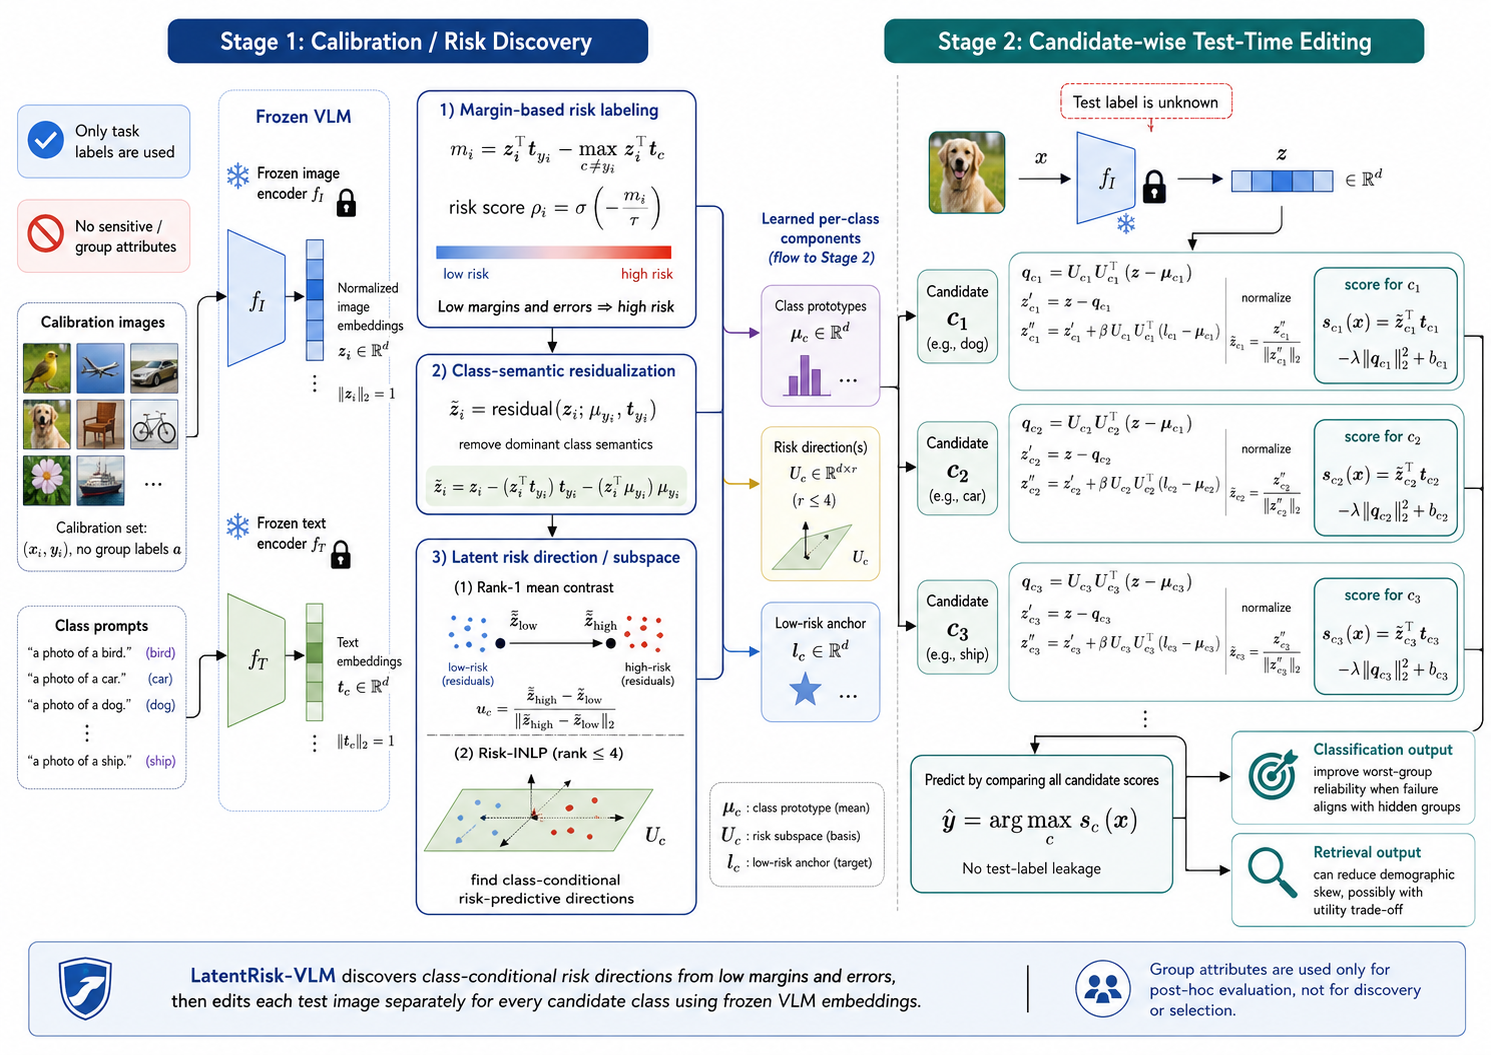
\includegraphics[width=\textwidth]{figures/picture.png}
\caption{\textsc{LatentRisk-VLM}. Risk directions are estimated from high- and low-risk residuals using mean contrast or iterative probes. At test time every candidate class is scored with its own correction; no test label selects the edit.}
\label{fig:pipeline}
\end{figure*}

\subsection{Removing Class-Level Semantics}
A risk estimator applied directly to $z_i$ may rely on ordinary
class-discriminative evidence rather than features genuinely associated
with classification error. For each class $c$, we therefore compute a
class prototype, defined as the mean embedding of its calibration samples:
\begin{equation}
 \mu_c=\frac{1}{|D_c|}\sum_{i:y_i=c}z_i,
\end{equation}
and form a residual orthogonal to the class text embedding:
\begin{equation}
 r_i=z_i-\mu_{y_i}, \qquad
 \tilde z_i=r_i-t_{y_i}t_{y_i}^{\top}r_i.
 \label{eq:residual}
\end{equation}
Subtracting the class prototype restricts risk-direction discovery to
within-class variation, while the second operation reduces the direct coupling between the representation and the corresponding class-prompt direction. However, these operations do not guarantee that all class information has been completely removed.

\paragraph{Unified design objective.}
We aim to identify a risk direction, or risk subspace, \(U_c\) that captures error-related information while containing as little class-semantic information as possible, such that suppressing it does not impair the classification capability. A compact specification is

% \begin{equation}
% \begin{aligned}
% \min_{U_c,\,\hat z^{(c)}}\quad
% &\mathcal{L}_{\mathrm{risk}}(U_c;\tilde Z_c,h_c) 
%  +\alpha\|t_c^{\top}U_c\|_2^2\\
% &\qquad +\lambda\|U_cU_c^{\top}(z-\mu_c)\|_2^2 -\hat z^{(c)\top}t_c\\
% \text{s.t.}\quad &U_c^{\top}U_c=I,\operatorname{rank}(U_c)\le r,\hat z^{(c)}=\operatorname{Edit}(z;U_c,\ell_c).
% \end{aligned}
% \label{eq:unified_objective}
% \end{equation}

\begin{equation}
\begin{aligned}
\min_{U_c,\,\hat z^{(c)}}\quad
&\mathcal{L}_{\mathrm{risk}}(U_c;\tilde Z_c,h_c)
+\alpha\|t_c^{\top}U_c\|_2^2\\
&\qquad+\lambda\|U_cU_c^{\top}(z-\mu_c)\|_2^2
-\hat z^{(c)\top}t_c .
\end{aligned}
\label{eq:unified_objective}
\end{equation}

Here, \(U_c^{\top}U_c=I\),\(\operatorname{rank}(U_c)\le r\), \(\hat z^{(c)}=\operatorname{Edit}(z;U_c,\ell_c)\).

% The first let found $U_C$ can predict risk. The second discourages class-semantic coupling. If this value is big, it means the risk direction is highly consistent with class text diretion, which means model learn class information rather than risk information. The third penalizes the candidate's risk activation. Project the features of the prototype samples of the removed category onto the risk subspace. If this value is large, it indicates that the sample contains a strong risk direction. Therefore, during the optimization process, we aim to reduce this activation. The fourth retains task semantics.Edited image embedding $\hat z^{(c)\top}$ still should maintain a high degree of similarity with the category text $t_c$. For constraint condition, \(U_c^{\top}U_c=I\) means the column vectors of $U_c$ are orthogonal.$U_c=[u_1,u_2,...,u_r]$ and $u_i^Tu_j=0$.\(\operatorname{rank}(U_c)\le r\) means only search for low-dimensional risk subspaces.\(\hat z^{(c)}=\operatorname{Edit}(z;U_c,\ell_c)\). Here $\operatorname{Edit}$ denotes the normalized candidate-wise projection and reinjection in Equations~\ref{eq:projection}--\ref{eq:score}, remove the risk direction through projection, and then inject neutral information. This is a design objective rather than an additional jointly optimized loss. In the implementation, class residualization reduces the semantic-coupling term, mean contrast or Risk-INLP estimates the risk term, projection implements suppressibility, and neutral reinjection plus the semantic score preserves utility. The scoring grid selects the operating point; $\alpha$ is not separately tuned.

The first term encourages the learned \(U_c\) to predict calibration risk. The second discourages coupling between the risk subspace and the class semantics. A large value of \(\|t_c^{\top}U_c\|_2^2\) indicates that the learned risk directions are strongly aligned with the class text embedding, suggesting that the model may be capturing class-discriminative information rather than risk-related information. The third term penalizes the candidate's activation in the risk subspace. Specifically, \(U_cU_c^{\top}(z-\mu_c)\) projects the class-centered feature onto the risk subspace. A large norm indicates that the candidate contains a strong risk component; therefore, the objective encourages this activation to be reduced. The fourth term preserves task semantics by encouraging the edited image embedding \(\hat z^{(c)}\) to remain highly similar to the class text embedding \(t_c\).

Regarding the constraints, \(U_c^{\top}U_c=I\) requires the columns of \(U_c\) to be orthonormal. In other words, for \(U_c=[u_1,u_2,\ldots,u_r]\), we have \(u_i^{\top}u_j=0\) for \(i\neq j\) and \(u_i^{\top}u_i=1\). The constraint \(\operatorname{rank}(U_c)\le r\) restricts the search to a low-dimensional risk subspace. Finally, \(\hat z^{(c)}=\operatorname{Edit}(z;U_c,\ell_c)\), where \(\operatorname{Edit}\) denotes the normalized candidate-wise projection and reinjection defined in Equations~\ref{eq:projection}--\ref{eq:score}: the risk component is first removed by projection, after which neutral information is reinjected.

This formulation is a design objective rather than an additional jointly optimized loss. In practice, class residualization reduces semantic coupling, mean contrast or Risk-INLP estimates the risk subspace, projection implements suppressibility, and neutral reinjection together with the semantic score preserves utility. The scoring grid determines the operating point, and \(\alpha\) is not tuned separately.

%  i think this can explain more clearly

\subsection{Estimating Risk Directions}
Let $H_c=\{i:y_i=c,h_i=1\}$ denote the set of high-risk or misclassified samples from class $c$, and let $L_c=\{i:y_i=c,h_i=0\}$ denote the corresponding low-risk or correctly classified samples. We estimate a class-specific risk direction by contrasting the mean residualized embeddings of these two groups:
\begin{equation}
 u_c=\frac{\bar z_{H_c}-\bar z_{L_c}}
 {\|\bar z_{H_c}-\bar z_{L_c}\|_2},
 \quad
 \bar z_S=\frac{1}{|S|}\sum_{i\in S}\tilde z_i.
 \label{eq:contrast}
\end{equation}
Here, $\bar z_{H_c}$ and $\bar z_{L_c}$ are the centroids of the high-risk and low-risk samples, respectively, in the residualized feature space. Their difference therefore points from the average representation of successful predictions toward that of failures. Normalizing this difference removes its scale and yields a unit vector that captures only the dominant direction of risk-related variation within class $c$.

Thus, $U_c=u_c\in\mathbb{R}^{d\times1}$ defines a one-dimensional, class-conditional risk subspace. For a residualized embedding $\tilde z_i$, the projection $u_c^\top \tilde z_i$ measures its activation along this direction, with larger values indicating greater alignment with the feature pattern associated with failures. The mean-contrast estimator provides the simplest linear description of how failures differ from successes after class residualization. Since it is constructed directly from the separation between high-risk and low-risk samples, it is risk-predictive by design. However, because no demographic or sensitive-attribute annotations are used, the resulting direction should be interpreted only as a latent risk direction rather than as a named demographic direction.

\paragraph{Probe-based directions.}
Alternatively, we fit a linear logistic probe to $h_i$ within each class. Its normalized weight becomes $u_{c,1}$; the residuals are projected into its null space, and the process repeats up to rank four or until probe accuracy falls below 0.55. QR orthogonalization yields $U_c=[u_{c,1},\ldots,u_{c,r}]$. This Risk-INLP estimator follows the iterative removal principle of \citet{ravfogel2020inlp}. Rank one tests a single discriminative direction, while rank four tests whether residual risk remains distributed after successive projections.

\subsection{Candidate-Wise Representation Editing}
For a test embedding $z$ and candidate class $c$, define its residual risk component $q_c=U_cU_c^\top(z-\mu_c)$. Full projection gives
\begin{equation}
 z'^{(c)}=z-q_c.
\label{eq:projection}
\end{equation}
Projection may move an embedding away from regions represented by low-risk calibration examples. Let $\ell_c$ be the mean original embedding over $L_c$. We reinsert half of its risk-subspace component,
\begin{equation}
 z''^{(c)}=z'^{(c)}+\beta U_cU_c^\top(\ell_c-\mu_c),
 \qquad \beta=0.5,
 \end{equation}
and normalize $\hat z^{(c)}=z''^{(c)}/\|z''^{(c)}\|_2$. The candidate score is
\begin{equation}
 s_c(x)=\hat z^{(c)\top}t_c-\lambda\|q_c\|_2^2+b_c.
 \label{eq:score}
\end{equation}
The first term retains CLIP semantic matching, the second penalizes candidate-specific risk activation, and $b_c$ is a class intercept. Prediction compares Equation~\ref{eq:score} over all $c$; it never applies a correction chosen by the ground-truth test class.

\subsection{Task-Label-Only Selection}
We choose $\lambda$ and $b_c$ on calibration data using accuracy (CelebA) or macro class accuracy (Waterbirds), with overall accuracy and smaller intervention parameters as tie breakers. Subspace rank, projection strength, and $\beta$ are fixed before this grid search. The primary selection score depends on $y$ but not $a$. For diagnosis, we rerun the same search using validation WGA over $(y,a)$ and label the resulting row \emph{attribute oracle}. Comparing the two selectors isolates a practical question: even if error-derived directions contain group-relevant information, can an attribute-free criterion choose a useful operating point?

\paragraph{Complexity.}
Using cached embeddings of dimension $d$, rank-1 discovery requires one pass over $n$ calibration samples, $O(nd)$ time and $O(nd)$ storage. Candidate-wise inference costs $O(|\mathcal{Y}|d)$ per image beyond the encoder call. The rank-$r$ extension increases projection cost to $O(|\mathcal{Y}|dr)$ and fits at most $r$ linear probes per class. No variant adds a VLM forward pass or modifies backbone parameters.

\subsection{Retrieval Adaptation}
For Flickr30K calibration captions, risk is the negative margin between the paired image and the hardest nonmatching image. Paired image embeddings are centered by their global prototype and residualized against their caption embeddings. Splitting at the median margin yields one high--low risk direction. The same projection and reinjection edit every gallery image, while $\lambda$ is selected by validation text-to-image Recall@10. The fitted editor is then evaluated unchanged on Flickr30K test retrieval and on FairFace demographic skew; FairFace gender labels never enter fitting or ranking.

\section{Experimental Protocol}
\paragraph{Backbone and reporting.}
All experiments use 768-dimensional, normalized embeddings from the Transformers CLIP ViT-L/14 implementation; both encoders are frozen. We report one deterministic run for each configuration. Results are measured adaptations to this common backbone, not numbers copied from the baseline papers.

\paragraph{Classification datasets.}
Waterbirds \citep{sagawa2020groupdro} uses the official validation split (1,199 images) for risk discovery and parameter selection and the test split (5,794 images) for evaluation. Fixed prompts are ``a photo of a landbird'' and ``a photo of a waterbird.'' Groups cross bird type with place. CelebA \citep{liu2015faceattributes} uses Blond Hair as the task and Male as the evaluation attribute. Its validation split (19,867 images) calibrates \textsc{LatentRisk-VLM}; its training split is available to fitted baselines; and its test split (19,962 images) is evaluated once. Prompts describe a person with or without blond hair.

\paragraph{Retrieval datasets.}
FairFace \citep{karkkainen2021fairface} supplies a 10,954-image validation gallery and the 25 gender-stereotype queries released with BEND-VLM. Its 86,744-image training split is used only as the gender-labeled reference bank for BEND-VLM. We report text-to-image retrieval on the Flickr30K \citep{young2014image} Karpathy test split \citep{karpathy2015deep}: 5,000 captions and 1,000 images. The 1,014-image validation split fits the LatentRisk retrieval editor. SANER is trained for five epochs on 124,026 person-related caption pairs from 27,576 disjoint Flickr30K training images.

\paragraph{Supervision accounting.}
We separate three classification settings. \emph{No example labels} includes frozen CLIP and prompt ensembling. \emph{Task labels only} includes ERM, JTT-style calibration, and the primary \textsc{LatentRisk-VLM} variants. \emph{Attribute-supervised or selected} includes any method that uses $a$ for adaptation, references, checkpoint choice, or validation-WGA selection: SPD, BEND-VLM, CFR, CnC, GIC, AFR, and our attribute oracle. This conservative accounting prevents validation access to $a$ from being presented as group-label-free.

\paragraph{Baselines.}
Classification evaluates frozen CLIP, prompt ensembling, ERM, JTT \citep{liu2021jtt}, AFR \citep{qiu2023afr}, CnC \citep{zhang2022correct}, BEND-VLM \citep{gerych2024bendvlm}, SPD \citep{zhao2026subspace}, CFR \citep{you2024calibrating}, and a GIC adaptation. Retrieval evaluates frozen CLIP, projection prompts \citep{chuang2023debiasing}, BEND-VLM, SANER \citep{hirota2025saner}, and \textsc{LatentRisk-VLM}. Where a reference method originally trains a different backbone, we retain its central objective and selection rule but operate on CLIP ViT-L/14 features or lightweight adapters. This creates a controlled frozen-backbone comparison, not an exact reproduction of each paper's original setting.

\paragraph{Hyperparameters.}
Classification uses $\tau=1$, $\eta=0.5$, full projection, and $\beta=0.5$. The measured rank-1 configuration uses mean contrast on Waterbirds and one logistic probe on CelebA; rank four uses iterative probes with $C=1$ and a 0.55 training-accuracy stopping threshold. Waterbirds searches 101 values of $\lambda\in[0,5]$ and 61 intercepts in $[-0.03,0.03]$; CelebA searches 51 values in $[0.05,0.30]$ over the same intercept grid. Retrieval searches 61 values of $\lambda\in[0,0.3]$ and selects $0.1$. The Waterbirds ablation changes one component at a time under task-label-only macro-accuracy selection.

\paragraph{Metrics.}
Classification reports average accuracy and WGA over the four $(y,a)$ groups. We also discuss their difference as the average--worst gap. Retrieval reports text-to-image Recall@10 and mean gender MaxSkew@100 over the 25 FairFace queries. MaxSkew compares retrieved gender proportions with a uniform target; lower is better. Group attributes are accessed only after prediction except in rows explicitly marked attribute-supervised.

\section{Measured Results and Analysis}
\subsection{Classification}
\begin{table*}[t]
\centering
\caption{Classification with frozen CLIP ViT-L/14 encoders, grouped by supervision. WGA, Avg., and Gap are worst-group accuracy, average accuracy, and their difference (percentage points). Attribute use for validation selection counts as attribute supervision.}
\label{tab:classification}
\scriptsize
\setlength{\tabcolsep}{3.2pt}
\resizebox{\textwidth}{!}{%
\begin{tabular}{@{}llccc ccc@{}}
\toprule
& & \multicolumn{3}{c}{Waterbirds} & \multicolumn{3}{c}{CelebA} \\
\cmidrule(lr){3-5}\cmidrule(lr){6-8}
Supervision & Method & WGA & Avg. & Gap & WGA & Avg. & Gap \\
\midrule
\multirow{2}{*}{No example labels}
 & Frozen CLIP & 33.6 & 83.7 & 50.1 & 71.5 & 78.2 & 6.7 \\
 & Prompt ensemble & 41.1 & 83.8 & 42.7 & 65.0 & 77.2 & 12.1 \\
\midrule
\multirow{4}{*}{Task labels only}
 & ERM & 29.4 & \textbf{86.6} & 57.2 & 16.1 & \textbf{94.3} & 78.2 \\
 & JTT-style calibration & 36.1 & 71.5 & 35.3 & 31.1 & 84.5 & 53.4 \\
 & \textsc{LatentRisk-VLM} (rank 1) & 60.5 & 78.4 & 17.9 & 54.4 & 91.7 & 37.3 \\
 & \textsc{LatentRisk-VLM} (rank 4) & 54.3 & 76.3 & 21.9 & 52.2 & 91.6 & 39.4 \\
\midrule
\multirow{7}{*}{Attribute-supervised/selected}
 & SPD (oracle attr.) & 22.7 & 77.2 & 54.4 & 67.7 & 77.8 & 10.2 \\
 & BEND-VLM & 31.0 & 81.2 & 50.2 & 58.6 & 73.5 & 14.9 \\
 & CFR & 47.7 & 74.4 & 26.7 & 9.7 & 39.0 & 29.3 \\
 & CnC & 32.9 & 83.8 & 50.9 & \textbf{85.3} & 87.5 & \textbf{2.3} \\
 & GIC-Cy + Subsample & 58.7 & 78.8 & 20.1 & 28.3 & 90.6 & 62.3 \\
 & AFR & 61.8 & 80.2 & 18.3 & 70.6 & 88.2 & 17.7 \\
 & \textsc{LatentRisk-VLM} (attr.-oracle selection) & 64.5 & 80.1 & 15.6 & 82.2 & 85.7 & 3.5 \\
\bottomrule
\end{tabular}%
}
\end{table*}

Table~\ref{tab:classification} reports the measured classification results. On Waterbirds, rank-1 \textsc{LatentRisk-VLM} is strongest among task-label-only methods at 60.5 WGA, improving frozen CLIP by 26.9 points while reducing average accuracy by 5.3 points. Among attribute-supervised or attribute-selected methods, our oracle reaches 64.5 WGA and AFR reaches 61.8. Thus the Waterbirds result supports failure-derived editing when the nuisance is unnamed, while exposing an explicit robustness--utility tradeoff.

CelebA reverses the primary result. Rank-1 editing raises average accuracy from 78.2 to 91.7 but lowers WGA from 71.5 to 54.4; rank four reaches 52.2 WGA. Changing only the rank-4 selection objective from validation accuracy to validation WGA raises test WGA by 30.0 points, from 52.2 to 82.2, while lowering average accuracy to 85.7. This oracle does not establish attribute-free robustness: it uses Male during selection and remains below the 85.3 WGA of attribute-selected CnC. The result instead isolates selection as a bottleneck after risk-subspace discovery.

\subsection{Retrieval Skew under Demographic Audit}
\begin{table}[t]
\centering
\caption{Measured retrieval with frozen CLIP ViT-L/14. MS@100 is mean gender MaxSkew@100 over 25 FairFace stereotype queries (lower is better). Flickr30K reports text-to-image Recall@10 on the Karpathy 1K test split (higher is better).}
\label{tab:retrieval}
\footnotesize
\setlength{\tabcolsep}{4pt}
\begin{tabular*}{\columnwidth}{@{\extracolsep{\fill}}lcc@{}}
\toprule
Method & MS@100 $\downarrow$ & R@10 $\uparrow$ \\
\midrule
Frozen CLIP & 0.355 & 92.2 \\
Projection prompts & 0.326 & \textbf{92.3} \\
BEND-VLM & \textbf{0.141} & 91.6 \\
SANER & 0.202 & 85.2 \\
\textsc{LatentRisk-VLM} & 0.323 & 88.2 \\
\bottomrule
\end{tabular*}
\end{table}

Table~\ref{tab:retrieval} shows that \textsc{LatentRisk-VLM} reduces FairFace MaxSkew from 0.355 to 0.323 while Flickr30K R@10 falls by 4.0 points. Projection prompts obtain a similar skew reduction without a utility loss. BEND-VLM obtains the lowest skew using gender-labeled FairFace training references. SANER uses predefined gender terms but no per-example attribute labels; it reduces skew further than \textsc{LatentRisk-VLM} while losing more retrieval utility. This binary-gender, 25-query audit does not establish general demographic debiasing.

\subsection{Ablation Study}
\begin{table}[t]
\centering
\caption{Waterbirds ablation with frozen CLIP ViT-L/14. Columns $y$ and $a$ indicate task- and attribute-label use. The last row is not a primary result.}
\label{tab:ablation}
\footnotesize
\setlength{\tabcolsep}{2.5pt}
\begin{tabular*}{\columnwidth}{@{\extracolsep{\fill}}lcccc@{}}
\toprule
Variant & $y$ & $a$ & Avg. & WGA \\
\midrule
Frozen CLIP & N & N & 83.7 & 33.6 \\
SPD (oracle attr.) & N & Y & 77.2 & 22.7 \\
\midrule
Single mean-contrast direction & Y & N & 78.4 & 60.5 \\
No semantic residualization & Y & N & 66.6 & 37.4 \\
No geometric suppression & Y & N & 77.0 & 57.1 \\
No risk-score penalty & Y & N & 76.3 & 54.3 \\
No neutral reinjection & Y & N & 76.3 & 54.4 \\
Full rank-4 editor & Y & N & 76.3 & 54.3 \\
\midrule
Rank 4 + attr.-oracle selection & Y & Y & \textbf{80.1} & \textbf{64.5} \\
\bottomrule
\end{tabular*}
\end{table}

Table~\ref{tab:ablation} shows that semantic residualization is necessary on Waterbirds: removing it lowers average accuracy from 76.3 to 66.6 and WGA from 54.3 to 37.4. Other components are not uniformly beneficial. Removing geometric suppression improves WGA from 54.3 to 57.1, and removing reinjection changes WGA by only 0.1 point. Validation macro accuracy selects $\lambda=0$ for the full rank-4 editor, making it identical to the no-risk-penalty row. Most importantly, mean contrast outperforms rank four by 2.1 average-accuracy and 6.2 WGA points. The evidence supports a simple direction on Waterbirds, not a general benefit from increasing rank.

\subsection{Risk Separability Is Insufficient}
On the calibration split, the Waterbirds mean-contrast directions separate risk labels with AUCs of 0.977 and 0.932 for landbirds and waterbirds. The CelebA rank-1 probes reach 0.989 and 0.981 for non-blond and blond classes. Yet the edits have opposite WGA effects. These are in-sample diagnostics, not generalization estimates, but they establish an important negative result: making failure linearly separable does not show that the direction corresponds to a hidden group or that removing it will improve group robustness.

\section{Discussion and Limitations}
\paragraph{Failure--group alignment is the key assumption.}
The method never identifies a group as such. It identifies representation variation associated with low margins within a class. Worst-group performance improves only when that variation overlaps the factor defining the worst group and can be removed without erasing class evidence. Waterbirds satisfies this condition strongly enough for rank 1; CelebA does not under task-only selection. Accordingly, \textsc{LatentRisk-VLM} should be described as latent-risk editing, not unsupervised demographic debiasing.

\paragraph{Discovery and selection are distinct.}
The CelebA oracle result is informative precisely because it is not a primary result. Group labels are absent from subspace discovery in both rows, yet changing only the validation objective produces a 30.0-point WGA difference. This shows that eliminating group labels from representation discovery does not eliminate the need for a deployment-relevant selection signal. Future work should target label-free robust selection, for example through stability across environments or tail-risk criteria, rather than assuming average accuracy will choose a fair edit.

\paragraph{Attribute supervision remains powerful.}
CnC outperforms our CelebA oracle under attribute-labeled validation. The appropriate comparison therefore depends on what is known at adaptation time. Latent-risk editing addresses an unnamed nuisance setting; it should not be presented as a replacement when reliable validation groups are available.

\paragraph{Experimental limitations.}
All results use one CLIP backbone and one deterministic run, so we cannot claim robustness across architectures or quantify seed variation. The classification datasets are binary, and the retrieval audit reduces gender to the binary labels supplied by FairFace and uses only 25 stereotype queries. The measured rank-1 estimator differs across classification datasets (mean contrast on Waterbirds and a logistic probe on CelebA), so their difference is not a fully controlled estimator comparison. Several baselines are adaptations to frozen CLIP features rather than exact reproductions in their original architectures and data regimes. The same validation split is used for risk discovery and parameter selection, which can favor calibration-specific structure. Finally, a predictive direction is correlational: these experiments do not establish that it causally generates errors or that editing it is safe under unmeasured shifts.

\paragraph{Ethical use.}
An attribute-free method can still worsen a protected group, as the CelebA result demonstrates. Aggregate accuracy must not be used to certify fairness, and post-hoc subgroup audits remain necessary whenever they are appropriate and lawful. The method should not be deployed to remove demographic information indiscriminately or to infer sensitive attributes. Its appropriate role is as an auditable representation intervention whose group consequences are measured explicitly.

\section{Conclusion}
We studied whether frozen-VLM failures can guide representation editing without group annotations. \textsc{LatentRisk-VLM} uses task-label margins, class residualization, risk-direction estimation, and candidate-wise inference without updating either encoder. It discovers error-related latent risk directions, not sensitive attributes or demographic groups. Rank-1 editing substantially improves CLIP Waterbirds WGA, while rank-4 editing with worst-class validation selection improves both CLIP Waterbirds and CLIP CelebA over task-accuracy selection. The SigLIP extension and the MetaShift-style cat/dog shift add a more cautious picture: changing the frozen backbone or shift can make task-accuracy selection fail badly, and rank-4 selection may recover WGA only with substantial average-accuracy tradeoffs or modest gains. Post-hoc diagnostics explain why rank-1 CelebA fails: the learned risk direction is stable but poorly aligned with the Male-defined spurious direction, and top-risk examples are not minority-enriched. The revised protocol positions CnC-Frozen, DFR-Frozen, INLP, and LEACE as supervised or attribute-budgeted frozen-feature adaptations rather than as full-backbone training costs. Methods with explicit attribute labels or group-aware validation remain stronger in settings where that supervision is available. Failure-derived directions are useful weak supervision when failure and hidden groups align, not a general substitute for group information.


\bibliography{latentrisk_vlm}

\end{document}
